\subsection{Sample via clustering}
\label{subsec:SampleViaClustering}

The choice of clustering methods to optimize \ac{cl} objectives 
arises naturally from the fact that positive pairs ought to be close 
to each other in the embedding space 
while samples of negative pairs ought to repel each other.
Intuitively, clusters of similar samples are considered positive samples.
Conversely, samples from different clusters are denoted negative samples.

Simple approaches, including \ac{drc} \citet{DRC_2020}, aim to create low intra-class diversity clusterings 
by considering both the \ac{af}, obtained from a \ac{cnn} with a fully connected layer, 
and the \ac{ap}, calculated via the softmax function of the \ac{af}, 
during clustering using a dedicated loss function.
This approach is motivated by their claim that existing methods cluster dissimilar \ac{af} together,
due to the usage of the maximum sensitivity of the softmax function used during cluster assignment.

Opposed to methods such as \ac{drc}, \ac{swav} does not directly encourage similar embeddings 
but similar 
cluster assignments for positive pairs \citet{swav_2020}.
The idea is to swap the assignments between two positive samples of the same image to encourage 
similar cluster assignments for similar instances.
A positive sample is obtained by applying a random augmentation to the anchor.

% interesting approaches
% Local Aggregation
\subsubsection{\acl{la}}\label{subsec:local_aggregation}

% s. unten: Hyperparameter prob- woher? k, H ist getestet, zumindest das Verhältnis, aber lambda wird aus anderer Arbeit übernommen -> keine Hyperparameter Suche

\citet{local_aggr_2019} optimize a low-dimensional feature space mapping by 
iteratively identifying close neighbours and updating the embedding function.
This soft clustering technique is called \ac{la}.

At each step during training of the embedding function $f_\theta: \mathcal{X} \rightarrow \mathcal{Z}$, 
two sets of neighbours are identified for each datapoint's embedding $z_i$ 
which are illustrated in \autoref{fig:la_bi_ci}.
The first set $C_i$ contains $z_i$'s close neighbours in the feature space, while
the second set $B_i$ contains $z_i$'s background neighbours.
$B_i$ is used as a means to judge distance and similarity, 
while $C_i$'s members should be embedded closer to $z_i$.
In other words, $C_i$ can be considered the set of positive samples while 
$B_i$ denotes the set of negative samples.
The level of \ac{la} $L(C_i,B_i | \theta, x_i)$ 
characterizes the relative level of closeness within $C_i$ compared to $B_i$.
$L(C_i,B_i | \theta, x_i)$ should be maximized.

The set $B_i$ consists of the $k$ nearest neighbours of $z_i$ in terms of cosine distance 
in the feature space.
$k$ is a hyperparameter and \citet{local_aggr_2019} set $k=4096$.
In order to construct $C_i$, 
first $H$ $k$-means clusterings are performed with sligthly different conditions.
Then, all of $z_i$'s clusters are united to form $C_i$.
$H$ and $k$ are hyperparameters.
\citet{local_aggr_2019} find that more clusterings, i.e. higher $H$, lead to isotropic clusters since outliers which arise from random processes are averaged out.
If $H$ is too high compared to the number of clusters $k$, the performance decreases.
They state that $H=3, k=10000$ and $H=10, k=30000$ are better values than $H=10, k=10000$ 
in terms of ResNet-18 nearest neighbour validation performance.

Finally, the level of \ac{la} $L(C_i,B_i | \theta, x_i)$ is defined as the negative log-likelihood 
of the feature space representation $z_i$ of $x_i$ being in $C_i$ given $B_i$, 
i.e., being recognized as a close neighbour given being recognized as a background neighbour.
The loss to minimize is $\mathcal{L} = L(C_i,B_i | \theta, x_i) + \lambda \left\| \theta \right\|^2$.
\citet{local_aggr_2019} choose to rely on hyperparameter settings from another work rather than conducting a hyperparameter search.

\begin{figure}[!htb] % h = here, t = top, b = bottom, p = page of floats
    \centering
    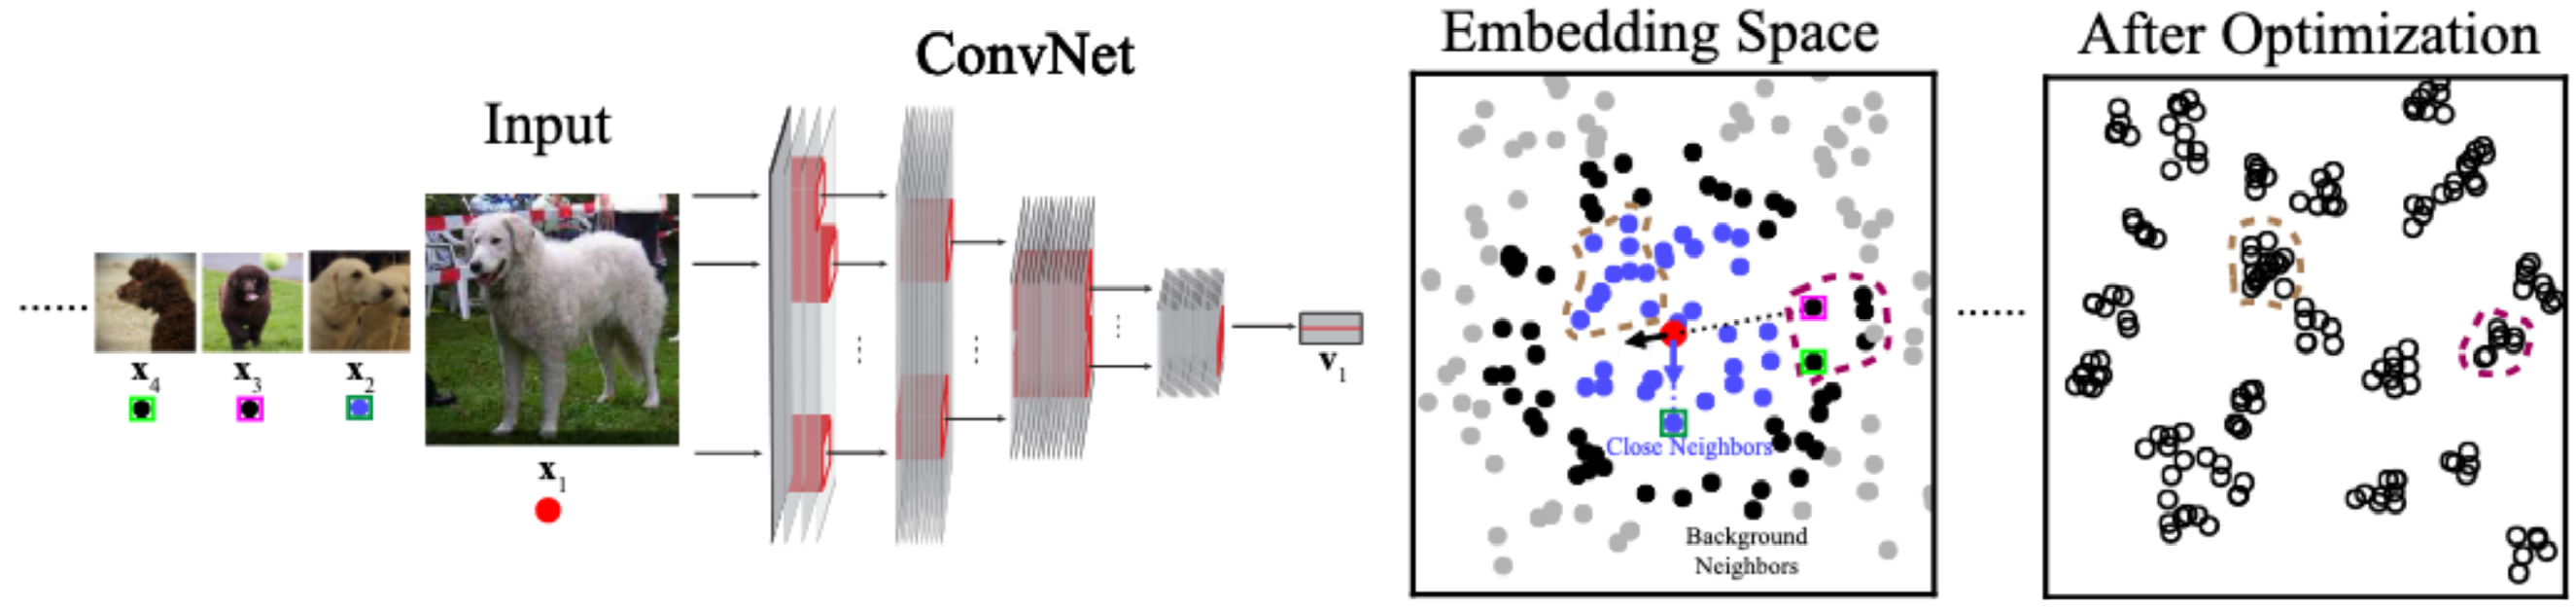
\includegraphics[width=360pt]{images/la_neighbourhoods.png}
    \caption{Illustration from \citet{local_aggr_2019}.
    A \ac{cnn} produces the feature space embedding $z_i = f_\theta(x_i)$.
    The embeddings are displayed as points in the feature space.
    The red point is the anchor $z_i$, 
    whereas blue points are close neighbours $C_i$ and
    black points are background neighbours $B_i$.
    The arrows denote influences between the neighbours.}
    \label{fig:la_bi_ci}
\end{figure}

% Mining on manifolds
\subsubsection{Mining on manifolds}\label{subsec:mining_manifolds}


% sparse usage of hard pairs inspired by SVMs

% purpose
According to \citet{mining_manifolds_2018}, the initial representation of the data is obtained by e.g. a pre-trained \ac{cnn}.
Hard pair mining is performed in order to fine-tune the network.

% idea of positive and negative samples
For fine-tuning, a combination of different definitions of proximity induces mining 
for hard positives and negatives as displayed in \autoref{fig:mining_manifolds_vis}.
Given an anchor, samples that reside on the same manifold but 
are not proximate in terms of Euclidean distance are considered hard positive samples.
These positive samples should be embedded closer to the anchor in the Euclidean space.
Conversely, hard negative samples are those that are spatially proximate in Euclidean space 
yet lie on different manifolds.
These samples should be embedded further away from the anchor in the Euclidean space.
%The hard samples are mined from an unordered set of \textit{relevant} samples.

% different neighbourhoods & hard samples
The authors denote the set of the $k$ nearest Euclidean neighbours $NN^e_k$ and 
the $k$ nearest manifold neighbours $NN^m_k$.
The hard positives are defined as $NN^m_k \textbackslash NN^e_k$. 
The pool $NN^m_k$ is ordered by descending manifold similarity to the anchor
to ensure that high-confidence samples are chosen first.
$k$ controls the diversity of the hard positives.
The larger $k$ is, the more diverse, i.e. hard, the hard positives are. 
The pool of hard negatives is defined as $NN^e_k \textbackslash NN^m_k$.
$NN^e_k$ is ordered by descending Euclidean distance to the anchor to keep the hardest samples.

% visualization of hard samples
\begin{figure}[!htb]% h = here, t = top, b = bottom, p = page of floats
    \centering
    \subfloat[\centering $k$ nearest Euclidean neighbour $NN^e_k$ (orange).]
    {{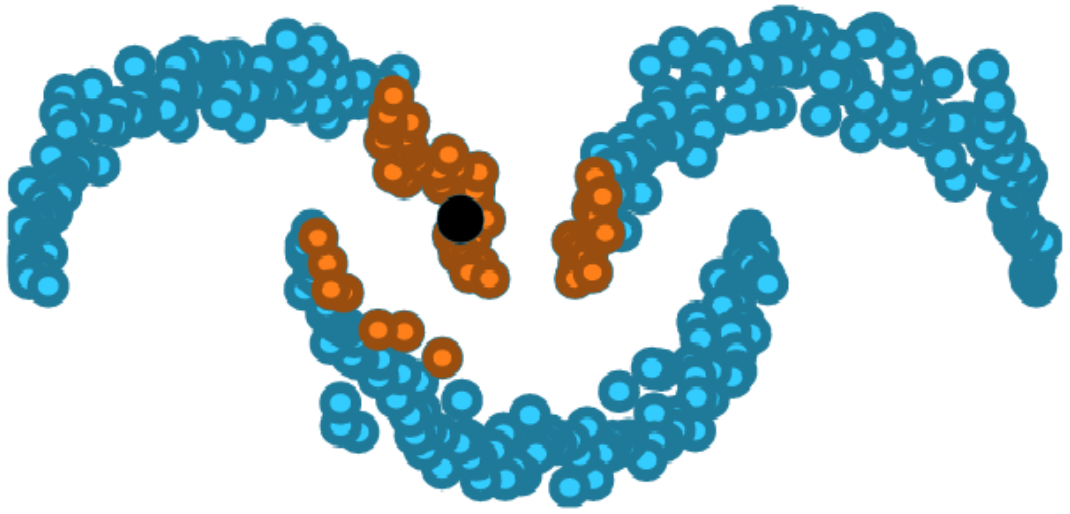
\includegraphics[width=5cm]{images/euclidean_NN.png} }}%
    \qquad
    \subfloat[\centering $k$ nearest manifold neighbour $NN^m_k$ (purple).]
    {{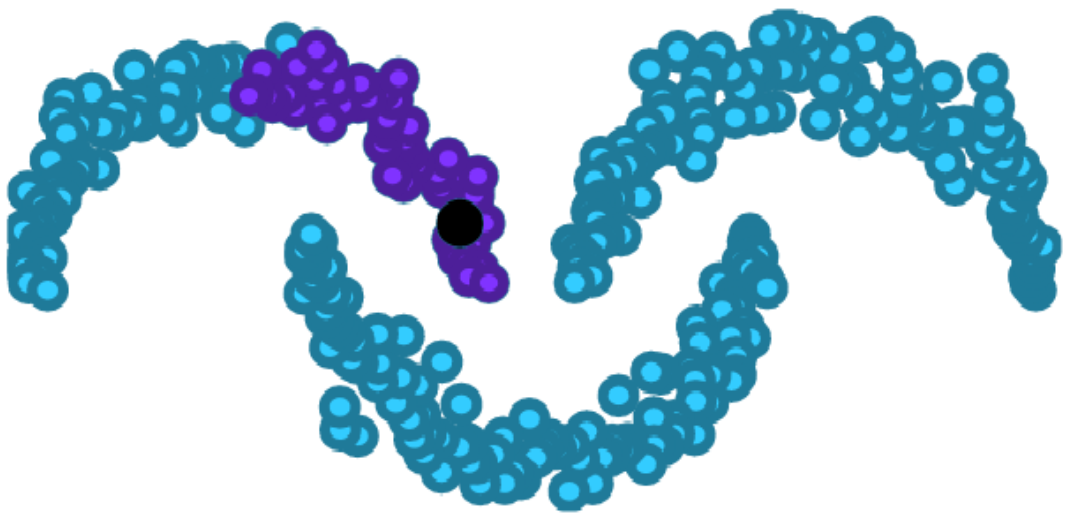
\includegraphics[width=5cm]{images/manifold_NN.png} }}%
    \qquad
    \subfloat[\centering Hard positives $NN^m_k \textbackslash NN^e_k$(green).]
    {{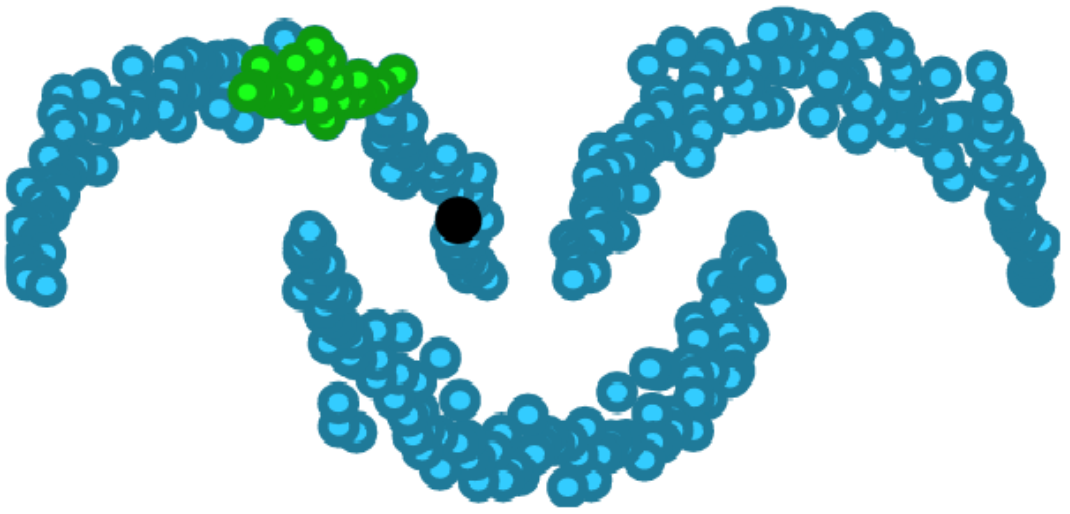
\includegraphics[width=5cm]{images/hard_positives_manifold.png} }}%
    \qquad
    \subfloat[\centering Hard negatives $NN^e_k \textbackslash NN^m_k$(red).]
    {{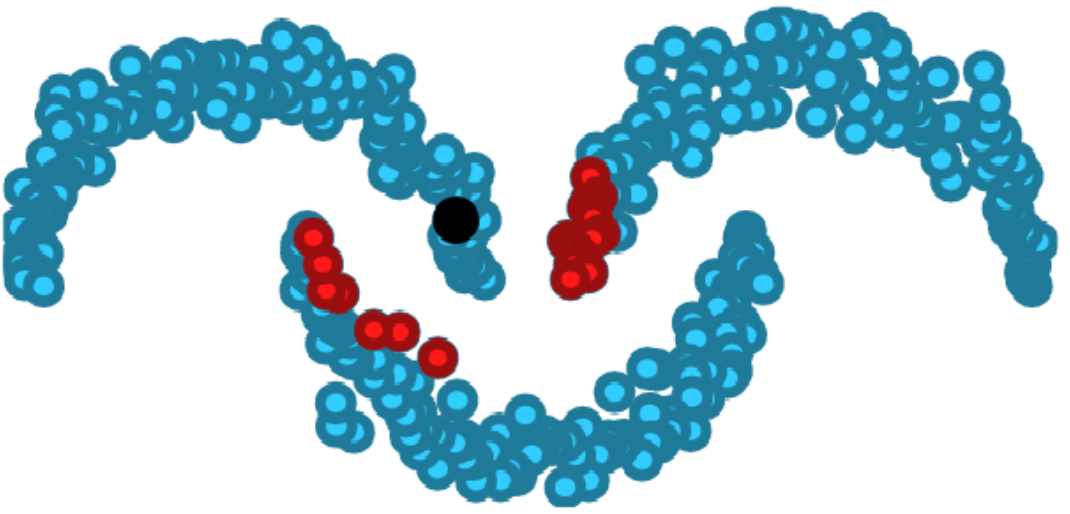
\includegraphics[width=5cm]{images/hard_negatives_euclidean.png} }}%

    \caption{Visualization of different proximity definitions, 
    the hard negatives and positives from \citet{mining_manifolds_2018}.
    The anchor is the black point.}%
    \label{fig:mining_manifolds_vis}%
\end{figure}


% manifolds via random walk n nearest neighbour graph
\citet{mining_manifolds_2018} propose a method where the manifold is estimated by mode-seeking, i.e. a random walk process, 
on the Euclidean nearest neighbour graph induced by the Euclidean similarity function $s_e$.
The graph is undirected, weighted and represented by a sparse symmetric adjacency matrix.
The adjacency matrix is constructed from the reciprocal $k$ nearest neighbours of each sample, 
where two points are considered reciprocal if each belongs to the $k$ nearest neighbours of the other. 
To reduce the negative impact of outliers, only reciprocal nearest neighbours are incorporated \citep{diffusion_2017,mining_manifolds_2018,fast_2018}.
The weighted adjacency matrix entries $a_{ij}$ defined in \Eqref{eq:mining_manifolds_adjacency_matrix} from \citet{mining_manifolds_2018} 
are calculated via the Euclidean distance between the samples if both nodes are in each other's nearest neighbourhood.
Diagonal entries are set to zero \citep{mining_manifolds_2018,fast_2018}.
%They admit that assessing the manifold similarity poses additional computational and memory requirements.
The manifold is computed once at the beginning \citep{mining_manifolds_2018}.

\begin{equation}
    a_{ij} = \begin{cases}
        s_e(y_i,y_j), & \text{if } y_i \in NN^e_k(y_j)\wedge y_j \in NN^e_k(y_i)\\
        0, & \text{otherwise}\\
      \end{cases}     
    \label{eq:mining_manifolds_adjacency_matrix}
\end{equation}


% mode seeking
% The manifold representation is obtained via mode-seeking as described in \citet{mode_seeking_2012}.
% The nearest neighbour network consists of samples as nodes and is weighted by the Euclidean distance 
% if both samples are in each other's $k$ nearest neighbourhood \citet{mode_seeking_2012,mining_manifolds_2018}.

% authority modes
While traditional mode-seeking relies on metric features, such as distances, mode-seeking on graphs 
uses the concept of random walks instead \citep{mode_seeking_2012}.
A random walk, i.e. a linear combination of the identity matrix and a scaled version of the adjacency matrix, is simulated multiple times on the graph.
\citet{mode_seeking_2012} define the so-called authority modes on a graph 
as the most frequently visited nodes by random walks among their local neighbours.
They correspond to the local maxima of the underlying probability distribution of random walks over the graph.
% selection of anchors
Since the anchors should be diverse and relevant, they are chosen to be the authority modes \citep{mining_manifolds_2018}.

% authority score
Inspired by PageRank, the possibility of random jumps is included in order to ensure convergence to a stationary distribution. 
The probability of visiting a node is denoted by the authority score $\pi$ 
which is defined in \Eqref{eq:authority_score} from \citet{mode_seeking_2012} 
where $p(i,j)$ are the entries of the Markov transition matrix $P$.
$\pi(j)$ takes into account the probability of visiting a node $j$ from a node $i$ and 
the probability of a random jump from one of the nodes chosen uniformly at random.
\citet{mode_seeking_2012} set $\alpha$ to $0.9$. 
The authority score $\pi$ can be computed by, for instance, the power method \citep{mode_seeking_2012,PageRank_2004}.

\begin{equation}
    \pi(j) = \alpha \sum_{i \in \mathcal{V}}^{}  \pi(i)p(i,j) + (1-\alpha)\frac{1}{N} , \text{ where } p(i,j) = \frac{a_{ij} }{\sum_{k \in \mathcal{V}}^{}a_{ik} } 
    \label{eq:authority_score}
\end{equation}

% local neighbours on the manifold: node relevancy 
\citet{mode_seeking_2012} define node relevancy $\Psi(s,t)$ via \Eqref{eq:node_relevancy} where $d(s)$ denotes the out-degree of a node.
To incorporate the reachability of a node, the probability of reaching node $t$ from node $s$ in $k$ steps $p_k(s,t)$ is 
defined via the $k_{th}$ power of the Markov transition matrix $P$.
To support similar authority scores between neighbouring nodes, the exponential term including a weighting factor $\gamma$ is included.
$\Psi(s,t)$ is not symmetric and depends on the random walk step $k$.
The authors propose to use the node relevancy $\Psi(s,t)$ for a node $s$ to determine the manifold neighbours $N_\varepsilon^m(s)$ for $s$ 
via the usage of a threshold $\varepsilon$: 
$N_\varepsilon^m(s) =  \left\{ t \in \mathcal{V} | \Psi(s,t) > \varepsilon \right\} \cup \left\{ s \right\}$ \citep{mode_seeking_2012}.

\begin{equation}
    \Psi(s,t) = d(s) p_k(s,t) \exp(-\gamma \left\{  \pi(t) - \pi(s)  \right\}^2)\text{, where } d(s) = \sum_{j\in \mathcal{V}}^{}a_{sj}
    \label{eq:node_relevancy}
\end{equation}

% AAS
They propose the \ac{aas} as a nonparametric estimator of the authority modes.
A node $s$ is shifted to node $\mathcal{A}(s)$ calculated in \Eqref{eq:authority_ascent_shift}. 
This formula chooses the local neighbour $t$ of $s$ that maximizes the difference of the authority scores $\pi$.
The authors argue that the \ac{aas} is finite and converges since the graph is finite.
When \ac{aas} is completed, manifolds are represented as clusters.
% examples
Resulting hard positives and negatives are displayed in \autoref{fig:manifold_mining_qualitative_analysis} and \autoref{fig:manifold_mining_examples}.

\begin{equation}
    \mathcal{A}(s) = \underset{t \in \mathcal{N_\varepsilon}(s)}{\text{argmax}} \left\{ p_k(s,t)\left[ \pi(t)-\pi(s) \right] \right\}
    \label{eq:authority_ascent_shift}
\end{equation}

% inlier and outlier
% Inliers on the manifold reside in large clusters while outliers are isolated in small groups since they do not have enough relevancy with inliers \citet{mode_seeking_2012}.
% Hence, outlier clusters can be identified by low sums of authority values.


\begin{figure}[!htb] % h = here, t = top, b = bottom, p = page of floats
    \centering
    \includegraphics[width=300pt]{images/mining_manifold_qualitative_analysis.png}
    \caption{Illustration of CUB200-2011 from \citet{mining_manifolds_2018}.
    The anchor is denoted $x^r$.
    A selection of hard positives from $P^+(x^r)$ is compared to the 
    baseline approach that samples from the closest neighbours to $x^r$ in 
    terms of Euclidean distance.
    Analogously, a selection of hard negatives from $P^-(x^r)$ 
    is compared to the baseline $X \textbackslash NN^e_3$, 
    i.e. sampling from the set that contains all samples but the three closest ones in 
    terms of Euclidean distance.
    The borders of the images denote the ground-truth class, i.e. if bird species is the same.
    Green borders indicate that the image belongs to the same class as the anchor, 
    while red borders signify images from a different class.
    It becomes apparent that the sampled hard positives consist of fewer false positives 
    than the baseline.
    }
    \label{fig:manifold_mining_qualitative_analysis}
\end{figure}

\begin{figure}[!htb] % h = here, t = top, b = bottom, p = page of floats
    \centering
    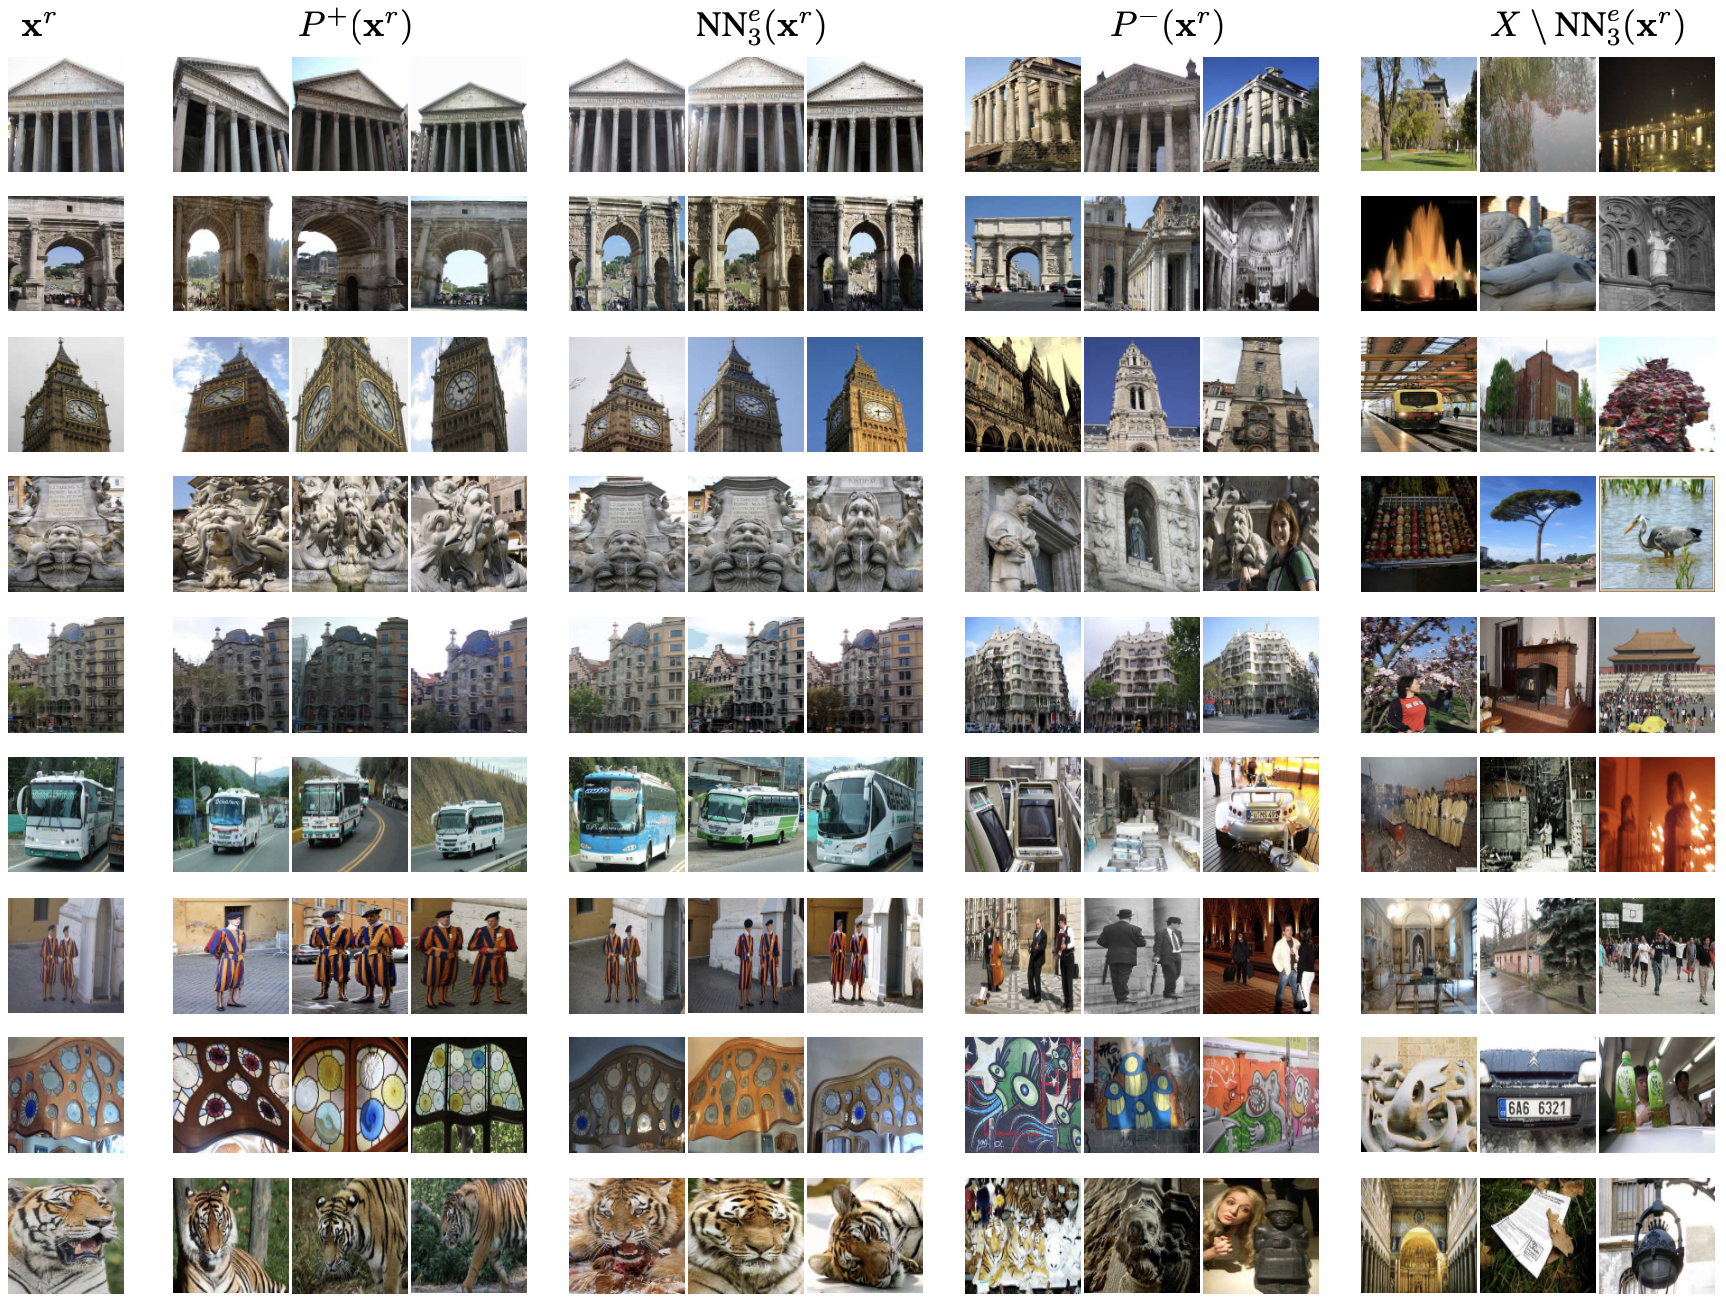
\includegraphics[width=360pt]{images/mining_manifold_examples.png}
    \caption{Illustration Oxford5k and Paris6k images crawled from Flickr from \citet{mining_manifolds_2018}.
    The dataset contains multiple images for each landmark building, i.e. class \citep{manifold_dataset}.
    The anchor is denoted $x^r$.
    A selection of hard positives from $P^+(x^r)$ is compared to the 
    baseline approach that samples from the closest neighbours to $x^r$ in 
    terms of Euclidean distance.
    Analogously, a selection of hard negatives from $P^-(x^r)$ 
    is compared to the baseline $X \textbackslash NN^e_3$, 
    i.e. sampling from the set that contains all samples but the three closest ones in 
    terms of Euclidean distance.
    It becomes apparent that the hard negatives display visually similar but 
    semantically different images to the anchor. % good
    }
    \label{fig:manifold_mining_examples}
\end{figure}

% loss functions
The authors propose multiple loss functions to train the model.
They, for instance, apply the contrastive loss $l_c(x^r, x^+, x^-)= \left\| x^r - x^+ \right\|^2 + \left[ m - \left\| x^r - x^- \right\| \right]^2$, 
the triplet loss $l_t(x^r, x^+, x^-)= \left[ m +  \left\| x^r - x^+ \right\| ^2 - \left\| x^r - x^- \right\| \right]^2$, 
and weighted versions of both contrastive and triplet loss, where the loss is multiplied by the manifold similarity of anchor and positive sample \citep{mining_manifolds_2018}.
$m$ is a margin parameter and $x^r$ is the representation of the anchor.

%PCL
\subsubsection{\acl{pcl}}\label{subsec:PCL}

\citet{PCL_2021} use clustering in the feature space to optimize the sample's representation.
Each sample is associated with $M$ prototypes, which are obtained through $k_m$-means clustering across various values of $m$.
These prototypes, represented by cluster centroids, act as latent variables and are classified as positive samples. 
A contrastive loss is applied to ensure that the sample's embedding aligns closely with its assigned prototypes.
The so-called prototypical contrastive loss ProtoNCE is optimized using an \ac{em} algorithm 
as displayed in \autoref{fig:PCL_training}.

\begin{figure}[!htb] % h = here, t = top, b = bottom, p = page of floats
    \centering
    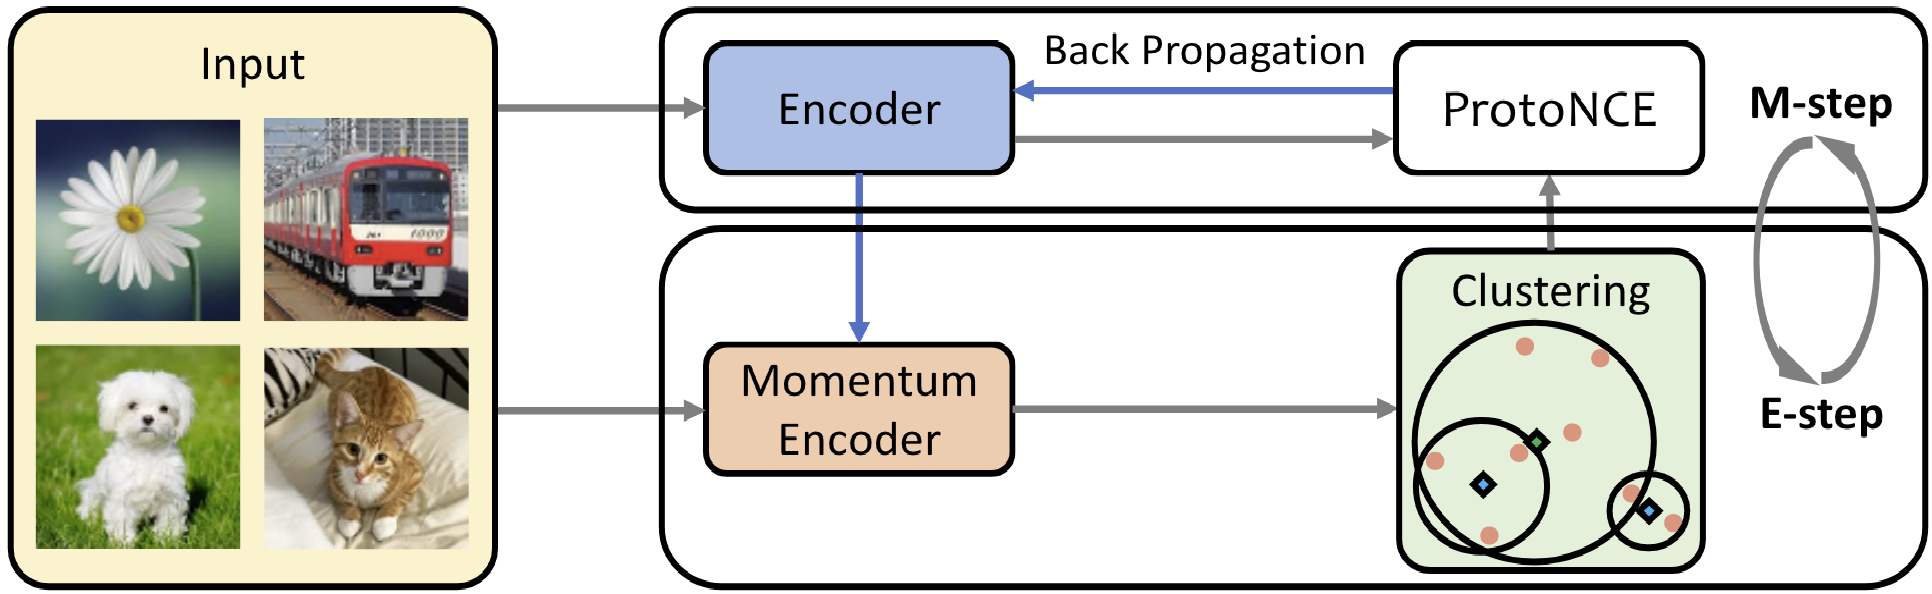
\includegraphics[width=360pt]{images/PCL_training.png}
    \caption{Illustration from \citet{PCL_2021}.
    The training process of the \ac{pcl} algorithm is demonstrated.
    $M$ $k_m$-means clusterings based on the feature space defined by the momentum encoder 
    are performed in the E-step.
    The prototypes $c^m_{\tilde{k}}$, $\tilde{k} \in [1, k_m]$, illustrated as green/ blue rectangles, 
    are the cluster centroids.
    The M-step updates the network parameters $\theta$ by optimizing the ProtoNCE loss.
    }
    \label{fig:PCL_training}
\end{figure}

% E-step: define k clusters & momentum encoder
$k$-means clustering is used to find the prototypes in the E-step.
The clustering is performed on the samples' embeddings obtained from the momentum encoder, 
whose parameters are a moving average of the main encoder's parameters and thus, smoother \citep{PCL_2021}.

% M-step
The M-step updates the network parameters $\theta$ by optimizing the ProtoNCE loss.
The minimization of the ProtoNCE loss is equivalent to maximizing the estimated log-likelihood.
The optimal parameters are those that map a sample close to its prototypes.
The result is obtained under the assumptions of a uniform prior over the cluster centroids, i.e. prototypes,
and an isotropic Gaussian distribution of the sample's embeddings around the prototypes.

% ProtoNCE loss
The ProtoNCE loss from \Eqref{eq:ProtoNCE} extends the InfoNCE from \Eqref{eq:InfoNCE} 
by not only enforcing similarity between the sample $z_i$ and 
one positive sample $z_i'$ while retaining dissimilarity to $r$ negative samples $z_j'$, 
but also considering its prototypes $c^m_s$. 
To enhance the stability of the results, $M$ clusterings are performed with varying numbers of clusters $k_m$. 
The use of different $k_m$ introduces varying levels of granularity among the prototypes, 
thereby encoding a hierarchical structure into the loss function.

\begin{equation}
    \mathcal{L}_{InfoNCE}= - \sum_{i=1}^{N}\log\frac{\exp \frac{z_i\cdot z_i'}{\tau}}{\sum_{j=0}^{r}\exp \frac{z_i\cdot z_j'}{\tau}}
    \label{eq:InfoNCE}
\end{equation}

\begin{equation}
    \mathcal{L}_{ProtoNCE}=\mathcal{L}_{InfoNCE} - \sum_{i=1}^{N} \frac{1}{M} \sum_{m=1}^{M} \log\frac{\exp \frac{z_i\cdot c_s^m}{\phi^m_s}}{\sum_{j=0}^{k_m}\exp \frac{z_i\cdot c_j^m}{\phi^m_j}}
    \label{eq:ProtoNCE}
\end{equation}


